\subsection{Матожидание}

    Давайте рассмотрим график матожидания \ref{EV} для модели с \(\beta\)-шумом, которая представлена формулой \ref{beta_chaos}. Мы видим, что на графике есть "выбросы" значений, например, такое можно увидеть на черной линии в точках \(\beta = 0.38\) и \(\beta = 0.45\). Для того, чтобы избавиться от таких выбросов и получить общую картинку происходящего далее будем анализировать усредненные матожидания.

    \comment{Думаю расписывать как построили усредненное матожидание не надо.}
        
    \begin{figure}
        \centering
        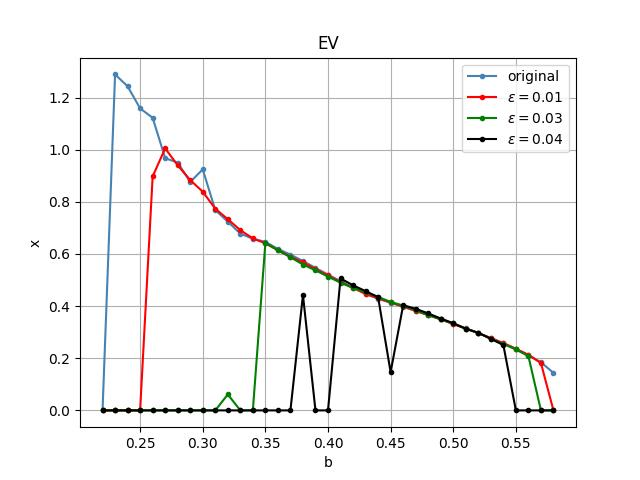
\includegraphics[width=\textwidth]{stochastic/images/EV.jpg}
        
        \captionsetup{justification=centering}
        \caption{Матожидание}
        \label{EV}
    \end{figure}

    Перейдем к рассмотрению графика \ref{EV_cyclic} усредненных значений математического ожидния. Мы видим, что нам удалось избавиться от "выборосов", описанных выше. При этом можно оценить \comment{что происходит на участкх, которые уходят вниз.}
        
    \begin{figure}
        \centering
        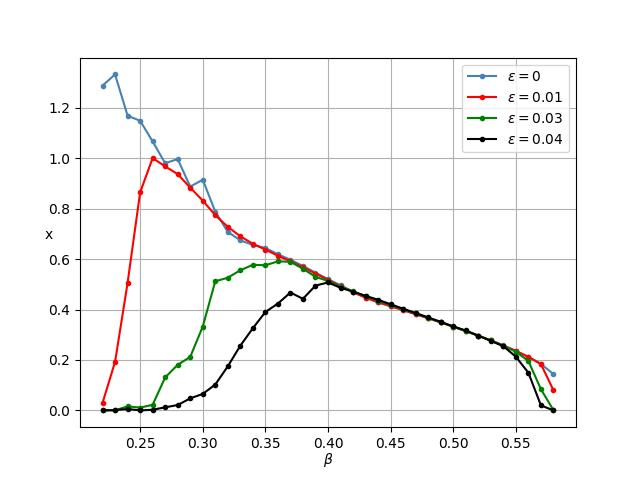
\includegraphics[width=\textwidth]{stochastic/images/EV_cyclic.jpg}
        
        \captionsetup{justification=centering}
        \caption{Циклическое матожидание}
        \label{EV_cyclic}
    \end{figure}

    На графике матожидания видно, что значения бифуркации при уменьшении параметра \(\beta\) растет, доходит до какого-то значения и сваливается в ноль. Заметим также, что при увеличении интенсивности наша модель начинает уходить в ноль при более больших значениях параметра \(\beta\). Это связано с тем, что при более высокой интенсивноти, шум оказывает более сильное влияние на развитие популяции.

    \comment{При чем, если есть шум, то уходим в ноль всегда, а при остуствии шума начинается зона хаоса}

    \comment{Точка начала сваливания в ноль обусловлена траекториями...}

    \comment{Теперь про касания...}

    \comment{А разные шумы?}